\documentclass[10pt]{article}
\usepackage{graphicx,float,latexsym,amsmath,amsfonts,amssymb,subeqnarray,colordvi,epstopdf,bbm}
\usepackage[latin1]{inputenc}
\usepackage{a4wide}

\def\re{{\Re}}
\def\R{\mathbb{R}}
\def\C{\mathbb{C}}
\def\imi{\textbf{\hskip1pt i\hskip1pt}}

\newtheorem{theorem}{Theorem}
\renewcommand{\thetheorem}{\thesection.\arabic{theorem}}
\newtheorem{lemma}[theorem]{Lemma}
\newtheorem{corollary}[theorem]{Corollary}
\newtheorem{proposition}[theorem]{Proposition}
\newtheorem{conjecture}[theorem]{Conjecture}
\newtheorem{assumption}[theorem]{Assumption}
\renewcommand{\theequation}{\thesection.\arabic{equation}}
\newenvironment{proof}{\noindent {\it Proof}~}{}
\newenvironment{proof2}[1]{\noindent {\it Proof} #1}{}
\newtheorem{remark}[theorem]{Remark}

\title{A Finite Volume Alternating Direction Implicit Approach for the Calibration of Stochastic Local Volatility models}
\author{Maarten Wyns\footnote{Department of Mathematics and Computer Science,
University of Antwerp, Middelheimlaan 1, B-2020 Antwerp, Belgium.
\mbox{Email}: \texttt{maarten.wyns@uantwerpen.be}.}
~and Jacques Du Toit\footnote{Numerical Algorithms Group, Oxford Street, Manchester, M1 5AN, United Kingdom. \mbox{Email}: \texttt{jacques@nag.co.uk}.}
}
\date{\today}

\begin{document}

\maketitle

\begin{abstract}
\noindent
In this paper ...
\end{abstract}
\vspace{0.2cm}\noindent
{\small\textbf{Key words:} TBD.}
\vspace{3mm}
\normalsize


%%%%%%%%%%%%%%%%%%%%%%%%%%%%%%%%%%%%%%%%%%%%%%%%%%%%%%%%%%%%%%%%%%%%%%%%%%%%%%%%%%%%
%%%%%%%%%%%%%%%%%%   SECTION 1   %%%%%%%%%%%%%%%%%%%%%%%%%%%%%%%%%%%%%%%%%%%%%%%%%%%
%%%%%%%%%%%%%%%%%%%%%%%%%%%%%%%%%%%%%%%%%%%%%%%%%%%%%%%%%%%%%%%%%%%%%%%%%%%%%%%%%%%%
\setcounter{equation}{0}
\section{Introduction}\label{intro}

In contemporary financial mathematics, \textit{stochastic local volatility} (SLV) models form state-of-the-art models to describe asset price processes, notably foreign exchange (FX) rates. In the latter situation one has to take into account two risk-free interest rates: one in the domestic currency, $r_{d}$, and one in the foreign currency, $r_{f}$. SLV models form a natural extension of \textit{local volatility} (LV) models, which can be described by the stochastic differential equation (SDE)
\begin{equation}
dS_{\tau} = (r_{d} - r_{f})S_{\tau} d\tau + \tilde{\sigma}_{LV}(S_{\tau},\tau) S_{\tau} dW_{\tau},
\label{eq:LVmodelS}
\end{equation}
where $S_{\tau}$ represents the exchange rate at time $\tau \ge 0$ and the value $S_{0}$ is given. The function $\sigma_{LV}(s,\tau)$ is called the \textit{local volatility function} and can be determined by the Dupire formula \cite{D94} such that the LV model reproduces the known market prices for European call and put options. In financial applications the local volatility function is often expressed as a function of $x= \log(s/S_{0})$. Moreover, the transformation $X_{\tau} = \log(S_{\tau}/S_{0})$ reflects better the duality between the exchange $S_{\tau}$ and $1/S_{\tau}$, where the latter one is the exchange rate when the role of the domestic currency and the foreign currency are swapped.
Define $\sigma_{LV}(x,\tau):=\tilde{\sigma}_{LV}(S_{0}\exp(x),\tau)$ and rewrite the SDE \eqref{eq:LVmodelS} as
\begin{equation}
dX_{\tau} = (r_{d} - r_{f} - \tfrac{1}{2} \sigma_{LV}^{2}(X_{\tau},\tau) ) d\tau + \sigma_{LV}(X_{\tau},\tau) dW_{\tau},
\label{eq:LVmodel}
\end{equation}
with $X_{0}=0$. Since the LV model is completely determined by the market prices of European call and put options, it offers no flexibility in matching the market dynamics. On the other hand, \textit{stochastic volatility} (SV) models are suited to reflect the market dynamics but they are often unable to capture the volatility smile. Both types of models can naturally be combined and extended to SLV models, see e.g.\ \cite{L02,TF10}. 
By combining features of the LV model with features of the SV models, SLV models are able to both match the market dynamics and reproduce the market prices for European call and put options. In this paper we consider SLV models of the type
\begin{equation}
\left\{ \begin{array}{l}
dX_{\tau} = (r_{d} - r_{f} - \tfrac{1}{2}\sigma^{2}_{SLV} (X_{\tau},\tau) \alpha^{2}(V_{\tau})) d\tau + \sigma_{SLV} (X_{\tau},\tau) \alpha(V_{\tau}) dW^{(1)}_{\tau}, \\\\
dV_{\tau} = \kappa (\eta - V_{\tau}) d\tau + \xi V_{\tau}^{\beta} dW^{(2)}_{\tau},
\end{array} \right.
\label{eq:SLVmodel}
\end{equation}
with $\alpha$ a non-negative function such that $\alpha(0)=0$, $\beta, \kappa, \eta, \xi$ strictly positive stochastic parameters, $dW^{(1)}_{\tau} \cdot dW^{(2)}_{\tau} = \rho d\tau$, $-1 \leq \rho \leq 1$ and given spot values $X_{0}=0, V_{0}$. Note that the process $V_{\tau}$ is always non-negative. In \cite{AP06} it is shown that the boundary $V_{\tau}=0$ is attainable for $0<\beta<1/2$ and for $\beta=1/2$ if $2\kappa \eta < \xi^2$. For $\beta>1/2$ it holds that $V_{\tau}=0$ is an unattainable boundary. Furthermore, $V_{\tau} = \infty$ is an unattainable boundary for all values of $\beta>0$.
Note that the choice $\alpha(v)=\sqrt{v}, \beta = 1/2$ corresponds to the Heston-based SLV model and the choice $\alpha(v)=v, \beta = 1$ corresponds to the SLV model described in \cite{TF10}.

In practical applications, one will first determine stochastic parameters that match the current market dynamics. Afterwards, the \textit{leverage function} $\sigma_{SLV} (x,\tau)$ is calibrated such that the model reproduces the known market prices for European call and put options.
It is well-known, see e.g.\ \cite{G86,T11}, that both the LV model \eqref{eq:LVmodel} and the SLV model \eqref{eq:SLVmodel} define the same marginal distribution for $S_{\tau}$, and hence the same fair values for vanilla options, if
\begin{equation}
\sigma^{2}_{LV} (x,\tau) = \mathbb{E}[\sigma_{SLV}^{2} (X_{\tau},\tau)\alpha^{2}(V_{\tau}) \vert X_{\tau} = x] = \sigma_{SLV}^{2} (x,\tau)\mathbb{E}[\alpha^{2}(V_{\tau}) \vert X_{\tau} = x].
\label{eq:SigmatoMatch}
\end{equation}
Since the conditional expectation itself also depends on the leverage function, computing it is a highly non-trivial task. Denote by $p(x,v,\tau;X_{0},V_{0})$ the joint density of $(X_{\tau},V_{\tau})$. The conditional expectation can then be written as
\begin{equation}
\mathbb{E}[\alpha^{2}(V_{\tau}) \vert X_{\tau} = x] = \frac{\int_{0}^{\infty} \alpha^{2}(v) p(x,v,\tau;X_{0},V_{0})dv}{\int_{0}^{\infty} p(x,v,\tau;X_{0},V_{0})dv}.
\label{eq:CondExpec}
\end{equation}
It can be shown, see e.g.\ \cite{C11}, that the joint density function satisfies the forward Kolmogorov equation
\begin{equation}
\begin{array}{lll}
\tfrac{\partial}{\partial \tau} p &=& \tfrac{\partial^{2}}{\partial x^{2}} \left( \tfrac{1}{2} \sigma^{2}_{SLV}\alpha^{2}(v)p \right) + \tfrac{\partial^{2}}{\partial x \partial v} \left( \rho \xi \sigma_{SLV}\alpha(v)v^{\beta} p \right) + \tfrac{\partial^{2}}{\partial v^{2}} \left( \tfrac{1}{2} \xi^{2} v^{2\beta} p \right) \\\\
&& - \ \tfrac{\partial}{\partial x} \left( (r_{d}-r_{f}-\tfrac{1}{2}\sigma^{2}_{SLV}\alpha^{2}(v)) p \right) - \tfrac{\partial}{\partial v} \left( \kappa(\eta - v) p \right),
\end{array}
\label{eq:ForwardKolmogorov}
\end{equation}
for $x \in \mathbb{R}, v>0, \tau >0$ and with initial condition $p(x,v,0;X_{0},V_{0}) = \delta(x)\delta(v-V_{0})$ where $\delta$ denotes the Dirac delta function. Once the joint density $p$ is known, one can easily determine the leverage function by computing the integrals in \eqref{eq:CondExpec}. Once the leverage function $\sigma_{SLV}$ is known, the joint density function can be determined by solving the partial differential equation (PDE) \eqref{eq:ForwardKolmogorov}. Initially, however, both $p$ and $\sigma_{SLV}$ are unknown and by combining \eqref{eq:CondExpec} and \eqref{eq:ForwardKolmogorov} one ends up with a highly non-linear PDE. 
In this paper we will introduce a finite volume alternating direction implicit approach for the numerical solution of general forward Kolmogorov equations of the type \eqref{eq:ForwardKolmogorov}. 
The approach makes use of the general \textit{method of lines} (MOL), cf. \cite{HV03}.
Here, the PDE is first discretized in the spatial variables, yielding large systems of stiff ordinary differential equations (ODEs). These, so-called, \textit{semidiscrete systems} are subsequently solved by applying a suitable implicit time stepping method.
Afterwards, an iteration procedure is proposed in combination with time stepping to approximate the leverage function that satisfies \eqref{eq:SigmatoMatch}. The outline of the paper is as follows: $\ldots \ldots \ldots$


%%%%%%%%%%%%%%%%%%%%%%%%%%%%%%%%%%%%%%%%%%%%%%%%%%%%%%%%%%%%%%%%%%%%%%%%%%%%%%%%%%%%
%%%%%%%%%%%%%%%%%%   SECTION 2   %%%%%%%%%%%%%%%%%%%%%%%%%%%%%%%%%%%%%%%%%%%%%%%%%%%
%%%%%%%%%%%%%%%%%%%%%%%%%%%%%%%%%%%%%%%%%%%%%%%%%%%%%%%%%%%%%%%%%%%%%%%%%%%%%%%%%%%%
\setcounter{equation}{0}
\section{Spatial discretization by Finite Volume schemes}\label{FV}

In the general MOL approach, the PDE is first discretized in the spatial variables by for example finite difference or finite volume methods. In this section a spatial discretization is proposed for a general two-dimensional forward Kolmogorov equation of the type
\begin{equation}
\tfrac{\partial}{\partial \tau} p = \tfrac{\partial^{2}}{\partial x^{2}} \left(\tfrac{1}{2} \sigma_{1}^{2}p \right) + \tfrac{\partial^{2}}{\partial x \partial y} \left( \rho \sigma_{1} \sigma_{2} p \right) + \tfrac{\partial^{2}}{\partial y^{2}} \left(\tfrac{1}{2} \sigma_{2}^{2} p \right) - \tfrac{\partial}{\partial x} \left( \mu_{1} p \right) - \tfrac{\partial}{\partial y} \left( \mu_{2} p \right),
\label{eq:GeneralForward}
\end{equation}
with $x,v \in \R$, $\tau >0$, and where $\sigma_{1}, \sigma_{2}, \mu_{1}, \mu_{2}$ are real coefficient functions of $x, y$.
Moreover, the functions  $\sigma_{1}, \sigma_{2}$ are required to be non-negative and it is assumed that there exist values $X_{0}, Y_{0}$ such that the initial function is given by $p(x,y,0)=\delta(x-X_{0})\delta(y-Y_{0})$.
Due to the form of the coefficients it is possible that the spatial domain is naturally restricted. For example, if $\mu_{2}(x,y) = \kappa(\eta-y)$ and $\sigma_{2}(x,y) = \xi y^{\beta}$ with $\kappa, \eta, \xi, \beta$ strictly positive constants, then the domain in the $y$-direction is naturally restricted to $y \ge 0$, cf.\ equation \eqref{eq:ForwardKolmogorov}.
Since the solution of a forward Kolmogorov equation represents the density of an underlying stochastic process, conservation of mass is important and the use \textit{finite volume} (FV) schemes is appropriate. Forward Kolmogorov equations of the type \eqref{eq:GeneralForward} are, however, not in conservative form and hence straightforward application of standard FV schemes is not possible. Moreover, rewriting PDE \eqref{eq:GeneralForward} in conservative form would involve derivatives of the coefficient functions, which are not known in general practical applications. 
In this section, a FV-based discretization of the spatial derivatives in the non-transformed PDE \eqref{eq:GeneralForward} is introduced such that conservation of total mass is guaranteed.
We start by explaining the discretization for a general one-dimensional forward Kolmogorov equation, and then generalise it to the two-dimensional case.


\subsection{One-dimensional forward Kolmogorov equations} \label{1DKolmogorov}

Standard one-dimensional forward Kolmogorov equations are also not written in conservative form and their solutions represent density functions of underlying stochastic processes. In this subsection a FV-based discretization is introduced for the general one-dimensional equation 
\begin{equation}
\tfrac{\partial}{\partial \tau} p =  \tfrac{\partial^{2}}{\partial x^{2}} \left( \tfrac{1}{2} \sigma^{2}p \right) - \tfrac{\partial}{\partial x} \left( \mu p \right),
\label{eq:GeneralForward1D}
\end{equation} 
for $x\in \R$, $\tau >0$, where $\sigma, \mu$ are real functions of $x$, with $\sigma$ non-negative and with initial function given by $p(x,0) = \delta(x-X_{0})$ for some real $X_{0}$.
Spatial discretization by finite difference (FD) or FV methods is often applied on a finite Cartesian grid. By consequence, the spatial domain has to be truncated to $[X_{\min}, X_{\max}]$, where the boundaries are chosen sufficiently far away from $X_{0}$ such that the truncation error is negligible. 
Recall that the form of $\sigma, \mu$ can naturally restrict the spatial domain of the PDE to for example $x \ge 0$. 
In the latter case, the lower boundary is naturally defined as $X_{\min}=0$. 
Next, let $X_{\min} = x_{1} < x_{2} < \ldots < x_{m_{1}} = X_{\max}$ be spatial mesh points and define spatial mesh widths
$$ \Delta x_{i} = x_{i} - x_{i-1}, \qquad \mathrm{for} \ 2 \le i \le m_{1},$$
and $\Delta x_{1} = \Delta x_{m_{1}+1} = 0$.
Spatial discretization then leads to approximations $P_{i}(\tau)$ of $p(x_{i},\tau)$. The idea of FV methods with mass conservation consists of creating a spatial discretization such that 
\begin{equation}
\sum_{i=1}^{m_{1}} P_{i}(\tau) \frac{\Delta x_{i} + \Delta x_{i+1}}{2} = \mathrm{constant,} \qquad \mathrm{for} \ \tau \ge 0.
\label{eq:ConservationMass1D}
\end{equation}
%where $\Delta x_{i} = x_{i} - x_{i-1}$ and $\Delta x_{1} = \Delta x_{m_{1}+1} = 0$.
Denote by $\Omega_{i}$ the cell
\begin{equation}
\Omega_{i} = [x_{i} - 0.5\Delta x_{i}, x_{i} + 0.5\Delta x_{i+1}],
\end{equation}
and denote by $x_{i \mp 0.5}$ the boundaries of this cell. In particular $x_{0.5}=x_{1}=X_{\min}$ and $x_{m_{1}+0.5}=x_{m_{1}}=X_{\max}$. Next, denote by $\overline{p}(x_{i},\tau)$ the cell average
$$ \frac{2}{\Delta x_{i} + \Delta x_{i+1}} \int_{\Omega_{i}} p(x,\tau) dx, $$
which is also a second-order approximation of the point value $p(x_{i},\tau)$. For this cell averages it holds that
\begin{subeqnarray}
\frac{\Delta x_{i} + \Delta x_{i+1}}{2} \frac{\partial}{\partial \tau }\overline{p}(x_{i},\tau) &=& \left. \left[ - \frac{\partial}{\partial x} \left( \frac{1}{2} \sigma^{2} p \right) + \mu p \right] \right\vert_{x=x_{i-0.5}} \slabel{eq:FluxLeft} \\
&& - \ \left. \left[ - \frac{\partial}{\partial x} \left( \frac{1}{2} \sigma^{2} p \right) + \mu p \right] \right\vert_{x=x_{i+0.5}}. \slabel{eq:FluxRight}
\label{eq:Fluxes}
\end{subeqnarray}
The right hand side of \eqref{eq:FluxLeft} can be seen as the flux on the left side of the cell $\Omega_{i}$ and \eqref{eq:FluxRight} is the flux on the right side of the cell.

Analogously to standard FV methods, cf. \cite{HV03}, we define discretizations of the form 
\begin{equation}
P_{i}'(\tau) = \left[ f_{i-0.5}(\tau,P(\tau)) - f_{i+0.5}(\tau,P(\tau)) \right] \frac{2}{\Delta x_{i} + \Delta x_{i+1}},
\label{eq:GeneralDiscretization1D}
\end{equation}
where $P(\tau)$ is the vector containing all the approximations $P_{i}(\tau)$.
The $f_{i \pm 0.5}(\tau,P(\tau))$ are discretizations of the fluxes from \eqref{eq:Fluxes}.
Note that $f_{0.5}$, respectively $f_{m_{1}+0.5}$, corresponds with the flux at the boundary $X_{\min}=x_{1}$, respectively $X_{\max} = x_{m_{1}}$. Moreover, by performing a discretization of the form \eqref{eq:GeneralDiscretization1D} and by ignoring the boundary terms, conservation of mass is achieved naturally inside the computational domain. 

The convection part of the PDE \eqref{eq:GeneralForward1D} is written in conservative form. For the inner cell boundaries, i.e.\ for $x_{i-0.5}$ with $2 \le i \le m_{1}$, we consider the second-order central FV scheme, cf.\ \cite{HV03}, and define
\begin{equation}
f_{a,i-0.5}(\tau,P(\tau)) := \mu_{i-0.5} \frac{P_{i}(\tau) + P_{i+1}(\tau)}{2},
\end{equation}
where $\mu_{i-0.5}= \mu(x_{i-0.5})$. 
The diffusion part is not written in conservative form and hence it is not possible to apply standard FV schemes to this term. 
The idea of the second-order FV scheme for diffusion, see e.g.\ \cite{HV03}, is generalised by defining
\begin{equation}
f_{d,i-0.5}(\tau,P(\tau)) := -\left(\tfrac{1}{2} \sigma^{2}_{i} P_{i}(\tau) - \tfrac{1}{2} \sigma^{2}_{i-1} P_{i-1}(\tau)\right) \frac{1}{\Delta x_{i}},
\end{equation}
for $2 \le i \le m_{1}$, where $\sigma_{i} = \sigma(x_{i})$.
It is readily seen that 
$$  \left(\tfrac{1}{2} \sigma^{2}_{i}p(x_{i},\tau) - \tfrac{1}{2} \sigma^{2}_{i-1} p(x_{i-1},\tau)\right) \frac{1}{\Delta x_{i}} $$
is a second-order approximation of $ \tfrac{\partial}{\partial x} ( \tfrac{1}{2} \sigma^{2}p)\vert_{x=x_{i-0.5}}$ which explains the choice for this discretization.
For the discretization of the total PDE \eqref{eq:GeneralForward1D} define
\begin{equation}
f_{i - 0.5}(\tau,P(\tau)) = f_{d,i - 0.5}(\tau,P(\tau)) + f_{a,i - 0.5}(\tau,P(\tau)),
\end{equation} 
such that one ends up with
\begin{eqnarray}
P_{i}'(\tau) &=& \frac{\sigma^{2}_{i-1}P_{i-1}(\tau)}{\Delta x_{i} (\Delta x_{i} + \Delta x_{i+1})} - \frac{\sigma_{i}^{2}P_{i}(\tau)}{\Delta x_{i} \Delta x_{i+1}} + \frac{\sigma^{2}_{i+1}P_{i+1}(\tau)}{\Delta x_{i+1} (\Delta x_{i} + \Delta x_{i+1})} \label{eq:Discretization1DWithoutBoundary} \\ \nonumber \\
&& + \  \left[ \mu_{i-0.5} \frac{P_{i-1}(\tau)+P_{i}(\tau)}{2} - \mu_{i+0.5} \frac{P_{i}(\tau)+P_{i+1}(\tau)}{2} \right] \frac{2}{\Delta x_{i} + \Delta x_{i+1}}, \nonumber
\end{eqnarray}
for $ 2 \le i \le m_{1}-1$. Note that by applying the second-order central FD scheme for diffusion on non-uniform spatial grids, cf.\ \cite{IHF10}, on the term $\tfrac{\partial^{2}}{\partial x^{2}} ( \tfrac{1}{2} \sigma^{2}p)$, one would end up with the same discretization for the diffusion term.

To complete this semidiscretization, it also has to be defined at the boundaries of the truncated domain such that conservation of the total mass is guaranteed, i.e.\ such that \eqref{eq:ConservationMass1D} is satisfied.
Given that $p$ represents a density function, it follows that
%Assuming that $p$ represents a density function, which is the case in our application, it follows that
$$ \int_{-\infty}^{\infty} p(,x,\tau) dx = 1, \qquad \forall \tau > 0,$$
and hence
$$ \int_{-\infty}^{\infty} \left[ \tfrac{\partial}{\partial \tau} p \right] dx = \int_{-\infty}^{\infty} \left[ \tfrac{1}{2} \tfrac{\partial^{2}}{\partial x^{2}} \left( \sigma^{2}p \right) - \tfrac{\partial}{\partial x} \left( \mu p \right) \right] dx = 0. $$
This condition makes sure that the total mass of the density function remains constant during the process. 
Assuming that $[X_{\min},X_{\max}]$ is chosen sufficiently wide, the condition above can be approximated by
$$ \left. \left[ \tfrac{\partial}{\partial x} \left( \tfrac{1}{2} \sigma^{2}p \right) - \left( \mu p \right) \right]\right\vert^{x= X_{\max}}_{x=X_{\min}} = 0. $$
This reflects that the total flux over the entire interval $[X_{\min},X_{\max}]$ is zero. 
As stated above, for some choices of coefficient functions the spatial domain is naturally restricted. For example, if the PDE \eqref{eq:GeneralForward1D} is stemming from a non-negative process, $X_{\min}$ can be set equal to zero. The no-flux boundary condition above then still holds on the naturally restricted domain.

Theoretically it could be the case that there is a positive flux at one of the boundaries, and exactly the same negative flux at the other boundary. 
However, since the solution represents a density function, it is more realistic to impose that no mass is coming in or going out at each of the boundaries. It is assumed that the following boundary conditions hold
\begin{eqnarray*}
\left. \left[ \tfrac{\partial}{\partial x} \left( \tfrac{1}{2} \sigma^{2}p \right) - \left( \mu p \right) \right]\right\vert_{x=X_{\min}} &=& 0, \\\\
\left. \left[ \tfrac{\partial}{\partial x} \left( \tfrac{1}{2} \sigma^{2}p \right) - \left( \mu p \right) \right]\right\vert_{x=X_{\max}} &=& 0.
\end{eqnarray*}
To implement the first condition, a ghost point $x_{0}=x_{1}-\Delta x_{2}$ is introduced.
The corresponding value $P_{0}(\tau)$ can be defined by making use of extrapolation and the boundary condition above in the following way
\begin{equation}
\frac{1}{2} \sigma_{0}^{2} P_{0}(\tau) = \frac{1}{2} \sigma_{2}^{2} P_{2}(\tau) - 2 \mu_{1} P_{1}(\tau) \Delta x_{2}.
\label{eq:ExtrapolBoundary}
\end{equation}
For the discretization of the flux at $x_{0.5}=x_{1}=X_{\min}$ stemming from the diffusion part we use this approximation and define
$$ f_{d,0.5}(\tau,P(\tau)) = -\left(\tfrac{1}{2} \sigma^{2}_{2} P_{2}(\tau) - \tfrac{1}{2} \sigma^{2}_{0} P_{0}(\tau)\right) \frac{1}{2\Delta x_{2}} = -\mu_{1}P_{1}. $$
Note that if the approximations in the middle formula are replaced by their exact values $p(x_{0},\tau)$, $p(x_{2},\tau)$, then this formula yields a second-order approximation of $-\tfrac{\partial}{\partial x} \left( \tfrac{1}{2} \sigma^{2}p \right) \vert_{x=x_{1}}$.
Since the grid point $x_{1}$ coincides with the left boundary of the first cell, the flux on the boundary $X_{\min}$ stemming from the convection part can be approximated directly by using the approximation $P_{1}$,
$$ f_{a,0.5}(\tau,P(\tau)) = \mu_{1} P_{1}. $$
The total flux at the boundary $X_{\min}$ is then approximated by 
$$ f_{0.5}(\tau,P(\tau)) = f_{d,0.5}(\tau,P(\tau)) + f_{a,0.5}(\tau,P(\tau))=0, $$
which is the semidiscrete equivalent of stating that no mass is coming in or going out at the boundary.
One ends up with the discretization
$$ P_{1}'(\tau) = -f_{1.5}(\tau,P(\tau))\frac{2}{\Delta x_{1} + \Delta x_{2}} = -f_{1.5}(\tau,P(\tau))\frac{2}{\Delta x_{2}}. $$
The boundary condition at $X_{\max}$ can be handled analogously in order to get
$$ P_{M_{1}}'(\tau) = f_{m_{1}-0.5}(\tau,P(\tau)) \frac{2}{\Delta x_{m_{1}}}. $$ 
By performing the discretization of the boundary conditions in this way, it follows that \eqref{eq:ConservationMass1D} is fulfilled, i.e.\ the total numerical mass is kept constant. 

By combining the discretization at boundaries with \eqref{eq:Discretization1DWithoutBoundary}, it is readily seen that the total discretization can be written as a system of ODEs
\begin{equation}
P'(\tau) = A P(\tau)
\label{eq:ODE1D}
\end{equation} 
for $\tau > 0$, with given matrix $A$. 
Since the values $P_{i}(\tau)$ can be seen as approximations of the cell averages $\overline{p}(x_{i},\tau)$, it is natural to define the initial vector $P(0)$ as 
$$ P_{i}(0) = \left\{ \begin{array}{lll}
\tfrac{2}{\Delta x_{i} + \Delta x_{i+1}} & & \mathrm{if} \ X_{0} \in [x_{i-0.5}, \ x_{i+0.5}], \\\\
0 && \mathrm{else.}
\end{array} \right. $$
In general, the exact solution of the system of ODEs \eqref{eq:ODE1D} can not be computed analytically and one relies on numerical methods in order to approximate it. Since the discretization above always leads to stiff semidiscrete systems, suitable implicit time stepping schemes such as the Crank--Nicolson scheme are widely considered [references].

 

\subsection{Numerical experiment} \label{subsec:Experiment1D}

In this subsection the performance of the FV discretization is tested by applying it to a practical example. Consider the SDE \eqref{eq:LVmodelS} with a constant local volatility function $\sigma_{LV} = \sigma_{BS} > 0$ such that the model reduces to the classical Black--Scholes model. Then, the underlying density is known exactly and given by
\begin{equation}
p(s,\tau) = n(\log(s/S_{0}),\tau)\frac{1}{s}, \qquad \mathrm{for} \ s>0, \tau > 0,
\label{eq:DensityBS}
\end{equation}
where $n(x,\tau)$ is the density function of a normally distributed random variable with mean $(r_{d}-r_{f}-\tfrac{1}{2}\sigma_{BS}^{2})\tau$ and variance $\sigma_{BS}^{2}\tau$. The density function $p(s,\tau)$ from \eqref{eq:DensityBS} satisfies the PDE
$$ \tfrac{\partial}{\partial \tau} p = \tfrac{\partial^{2}}{\partial s^{2}} \left( \tfrac{1}{2} \sigma_{BS}^{2}s^{2}p \right) - \tfrac{\partial}{\partial s} \left( (r_{d} - r_{f})s p \right), $$
for $s, \tau > 0$, with $p(s,0)=\delta(s-S_{0})$. This PDE is of the form \eqref{eq:GeneralForward1D} with a natural restriction of the spatial domain. Note that for the numerical experiment we don't apply the $\log$-transformation from Section \ref{intro} in order to have non-constant coefficients which makes the problem more challenging.

Firstly, the spatial domain is truncated to $[S_{\min}, S_{\max}] = [0, 30S_{0}]$ and we define a non-uniform grid $s_{1} < s_{2} < \cdots < s_{m_{1}}$ by making use of a $\sinh$ transformation of a uniform underlying grid, cf. \cite{IHF10}. In Figure \ref{fig:Grid1D} the spatial grid is shown for the values $S_{0}=100, m_{1} = 40$ and from $s=0$ to $s=5S_{0}$ to illustrate the smaller mesh widths around the point $s=S_{0}$.
\begin{figure}
\begin{center}
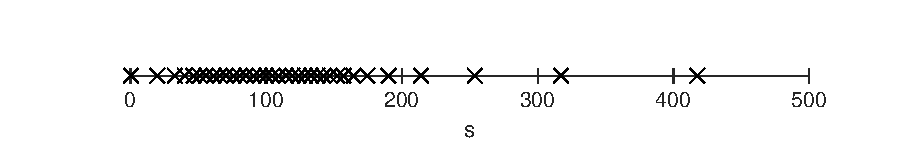
\includegraphics[scale=0.5]{Grid1D.eps}  
\caption{Illustration of the non-uniform grid around $S_{0}$ for the actual values $S_{0}=100, m_{1}=40$.}
\label{fig:Grid1D}
\end{center}
\end{figure}
After applying the FV discretization from Subsection \ref{1DKolmogorov}, we compute the total spatial error
$$ \max_{1 \le i \le m_{1}} \vert p(s_{i},T) - P_{i}(T) \vert. $$
In Figure \ref{fig:Convergence1D} the total spatial error is shown for the practical situation where $r_{d} = 0.03$, $r_{f} = 0.01$, $\sigma_{BS} = 0.2, T=1$ and for the number of spatial grid points $m_{1} = \{ 20, 40, \ldots, 200\}$. 
The convergence plot clearly indicates that the FV discretization is second-order convergent with respect to the current initial-boundary value problem.
\begin{figure}
\begin{center}
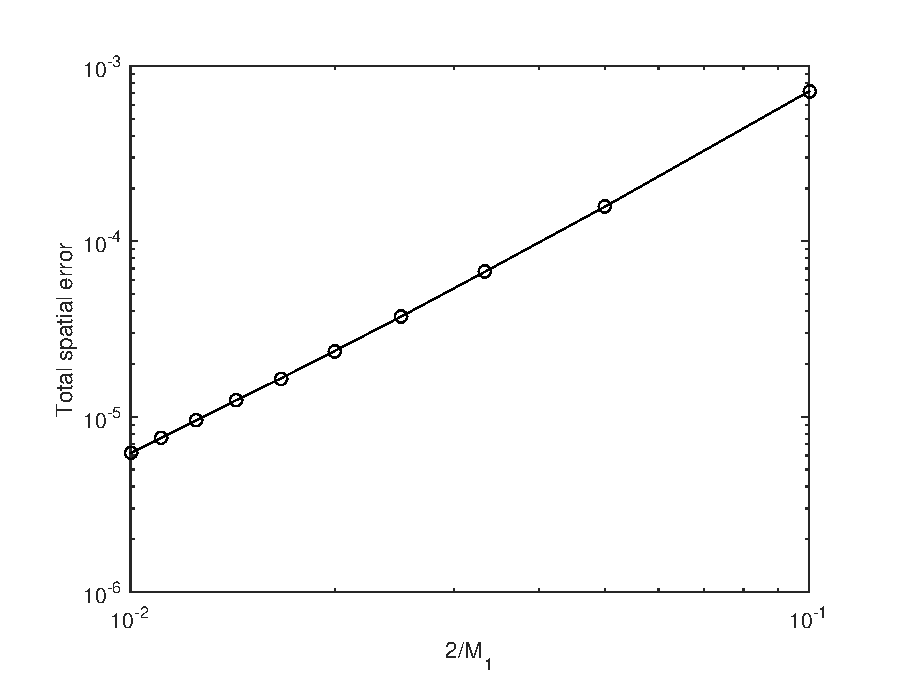
\includegraphics[scale=0.5]{Convergence1D.eps}  
\caption{Convergence plot for the practical situation where $r_{d} = 0.03, r_{f} = 0.01, \sigma_{BS} = 0.2, T=1$.}
\label{fig:Convergence1D}
\end{center}
\end{figure}



\subsection{Two-Dimensional forward Kolmogorov equations} \label{2DKolmogorov}

In this subsection, the FV discretization from the one-dimensional case is used to define a spatial discretization for the general two-dimensional forward Kolmogorov equation \eqref{eq:GeneralForward}. Suppose the spatial domain is truncated to $[X_{\min}, X_{\max}] \times [Y_{\min}, Y_{\max}]$, the spatial grid points in the $x$-direction, respectively $y$-direction, are given by
$$X_{\min} = x_{1} < x_{2} < \ldots < x_{m_{1}} = X_{\max},$$
respectively
$$Y_{\min} = y_{1} < y_{2} < \ldots < y_{m_{2}} = Y_{\max}.$$
Next, define spatial mesh widths $\Delta x_{i} = x_{i}-x_{i-1}$ and $\Delta y_{j} = y_{j}-y_{j-1}$ with $\Delta x_{1} = \Delta x_{m_{1}+1} = \Delta y_{1} = \Delta y_{m_{2}+1} = 0$.
Semidiscretization then leads to approximations $P_{i,j}(\tau)$ of $p(x_{i},y_{j},\tau)$.
Denote by $\boldsymbol{P}(\tau)$ the $m_{1} \times m_{2}$ matrix with entries $P_{i,j}(\tau)$ and let 
$$P(\tau) = \mathrm{vec}[\boldsymbol{P}(\tau)],$$ 
where $\mathrm{vec}[\cdot]$ denotes the operator that turns any given matrix into a vector by putting its successive columns below each other.
Analogously to the one-dimensional case, the solution of a two-dimensional forward Kolmogorov equation represents a density function and it is useful to keep the total numerical mass constant, i.e.\ to have
\begin{equation} 
\sum_{i=1}^{m_{1}} \sum_{j=1}^{m_{2}} \boldsymbol{P}_{i,j}(\tau) \frac{\Delta x_{i} + \Delta x_{i+1}}{2}\frac{\Delta y_{j} + \Delta y_{j+1}}{2}=\mathrm{constant,} \qquad \mathrm{for} \ \tau \ge 0. 
\label{eq:ConservationMass2D}
\end{equation}
Note that the weights corresponding with the point $(x,y)=(x_{i},y_{j})$ are equal to the area of the volumes
$$ \Omega_{i,j} := [x_{i-0.5}, x_{i+0.5}] \times [y_{j-0.5}, y_{j+0.5}], $$
where $x_{i \mp 0.5}$, respectively $y_{j \mp 0.5}$, are defined analogously as in the one-dimensional case.
Denote by $\vert \Omega_{i,j} \vert$ the area of the corresponding volume and by $\overline{p}(x_{i},y_{j},\tau)$ the volume average
$$ \frac{1}{\vert \Omega_{i,j} \vert} \int_{\Omega_{i,j}} p(x,y,\tau) dx dy, $$
which forms again a second-order approximation of the point value $p(x_{i},y_{j},\tau)$. It is readily verified that
\begin{subeqnarray}
\vert \Omega_{i,j} \vert \frac{\partial}{\partial \tau} \overline{p}(x_{i},y_{j},\tau) &=& \int_{y_{j-0.5}}^{y_{j+0.5}} \left. \left[ \frac{\partial}{\partial x} \left( \frac{1}{2} \sigma_{1}^{2} p \right) - \mu_{1}p \right] \right\vert_{x=x_{i-0.5}}^{x=x_{i+0.5}} dy \\
&& + \ \int_{x_{i-0.5}}^{x_{i+0.5}} \left. \left[ \frac{\partial}{\partial y} \left( \frac{1}{2} \sigma_{2}^{2} p \right) - \mu_{2}p \right] \right\vert_{y=y_{j-0.5}}^{y=y_{j+0.5}} dx \\
&& + \ \left. \left[ \left. \left[ \sigma_{1}\sigma_{2} p \right] \right\vert_{x=x_{i-0.5}}^{x=x_{i+0.5}} \right] \right\vert_{y=y_{j-0.5}}^{y=y_{j+0.5}}.
\end{subeqnarray}
The FV discretization is then based on the approximation
\begin{subeqnarray}
\frac{\partial}{\partial \tau} \overline{p}(x_{i},y_{j},\tau) &\approx& \left. \left[ \frac{\partial}{\partial x} \left( \frac{1}{2} \sigma_{1}^{2} p \right) - \mu_{1}p \right] \right\vert_{x=x_{i-0.5}}^{x=x_{i+0.5}} \frac{2}{\Delta x_{i} + \Delta x_{i+1}} \slabel{eq:FluxX} \\
&& + \ \left. \left[ \frac{\partial}{\partial y} \left( \frac{1}{2} \sigma_{2}^{2} p \right) - \mu_{2}p \right] \right\vert_{y=y_{j-0.5}}^{y=y_{j+0.5}} \frac{2}{\Delta y_{j} + \Delta y_{j+1}} \slabel{eq:FluxY} \\
&& + \ \left. \left[ \left. \left[ \sigma_{1}\sigma_{2} p \right] \right\vert_{x=x_{i-0.5}}^{x=x_{i+0.5}} \right] \right\vert_{y=y_{j-0.5}}^{y=y_{j+0.5}} \frac{2}{\Delta x_{i} + \Delta x_{i+1}} \frac{2}{\Delta y_{j} + \Delta y_{j+1}} . \slabel{eq:FluxXY}
\end{subeqnarray}
The terms in \eqref{eq:FluxX} and \eqref{eq:FluxY} are fluxes in one spatial dimension at the volume boundaries. The four terms included in \eqref{eq:FluxXY} can be seen as fluxes at the corners of the volume $\Omega_{i,j}$.
For the one-dimensional fluxes we generalise the FV schemes from the one-dimensional case. More precisely, the fluxes in the right hand side of \eqref{eq:FluxX} are discretized at the inner volume boundaries by
\begin{equation}
f_{i-0.5,j}(\tau,P(\tau)) = f_{d,i-0.5,j}(\tau,P(\tau)) + f_{a,i-0.5,j}(\tau,P(\tau)), \quad \mathrm{for} \ 2 \le i \le m_{1}, 1 \le j \le m_{2},
\end{equation}
where this time
\begin{equation}
\begin{array}{l}
f_{d,i-0.5,j}(\tau,P(\tau)) := -\left( \tfrac{1}{2} \sigma^{2}_{1,i,j} \boldsymbol{P}_{i,j}(\tau) - \tfrac{1}{2} \sigma^{2}_{1,i-1,j} \boldsymbol{P}_{i-1,j}(\tau) \right) \frac{1}{\Delta x_{i}}, \\\\
f_{a,i-0.5,j}(\tau,P(\tau)) := \mu_{1,i-0.5,j} \frac{\boldsymbol{P}_{i-1,j}(\tau)+\boldsymbol{P}_{i,j}(\tau)}{2},
\end{array}
\end{equation}
and $\mu_{1,i-0.5,j} = \mu_{1}(x_{i-0.5},y_{j})$, $\sigma_{1,i,j} = \sigma_{1}(x_{i},y_{j})$.
The spatial derivatives in the $x$-direction are then approximated by 
$$ \left[ f_{i-0.5,j}(\tau,W(\tau)) - f_{i+0.5,j}(\tau,W(\tau)) \right] \frac{2}{\Delta x_{i}+\Delta x_{i+1}}. $$
The fluxes in \eqref{eq:FluxY} at the inner volume boundaries are discretized in the same way by
\begin{equation}
f_{i,j-0.5}(\tau,P(\tau)) = f_{d,i,j-0.5}(\tau,P(\tau)) + f_{a,i,j-0.5}(\tau,P(\tau)), \quad \mathrm{for} \ 1 \le i \le m_{1}, 2 \le j \le m_{2},
\end{equation}
where
\begin{equation}
\begin{array}{l}
f_{d,i,j-0.5}(\tau,P(\tau)) := -\left( \tfrac{1}{2} \sigma^{2}_{2,i,j} \boldsymbol{P}_{i,j}(\tau) - \tfrac{1}{2} \sigma^{2}_{2,i,j-1} \boldsymbol{P}_{i,j-1}(\tau) \right) \frac{1}{\Delta y_{j}}, \\\\
f_{a,i,j-0.5}(\tau,P(\tau)) := \mu_{2,i,j-0.5} \frac{\boldsymbol{P}_{i,j-1}(\tau)+\boldsymbol{P}_{i,j}(\tau)}{2},
\end{array}
\end{equation}
and $\mu_{2,i,j-0.5} = \mu_{2}(x_{i},y_{j-0.5})$, $\sigma_{2,i,j} = \sigma_{2}(x_{i},y_{j})$. The spatial derivatives in the $y$-direction are approximated by
$$ \left[ f_{i,j-0.5}(\tau,P(\tau)) - f_{i,j+0.5}(\tau,P(\tau)) \right] \frac{2}{\Delta y_{j}+\Delta y_{j+1}}. $$
The fluxes from \eqref{eq:FluxXY} at the corners of the volumes, stemming from the mixed spatial derivative, are discretized in the following way for $1 \leq i \leq m_{1}+1, 1 \leq j \leq m_{2}$
\begin{equation} f_{m,i-0.5,j\pm0.5}(\tau,P(\tau)) = \sigma_{1,i-0.5,j\pm0.5}\sigma_{2,i-0.5,j\pm0.5} \frac{\boldsymbol{P}_{i-1,j}(\tau) + \boldsymbol{P}_{i-1,j\pm 1}(\tau)+\boldsymbol{P}_{i,j}(\tau)+\boldsymbol{P}_{i,j\pm 1}(\tau)}{4},  
\label{eq:DiscrMixedDerivative}
\end{equation}
where $\sigma_{1,i-0.5,j\pm0.5} = \sigma_{1}(x_{i-0.5},y_{j\pm0.5})$, $\sigma_{2,i-0.5,j\pm0.5} = \sigma_{2}(x_{i-0.5},y_{j\pm0.5})$, and
\begin{equation}
\boldsymbol{P}_{0,j}(\tau) := \boldsymbol{P}_{1,j}(\tau), \ \boldsymbol{P}_{m_{1}+1,j}(\tau):= \boldsymbol{P}_{m_{1},j}(\tau), \ \boldsymbol{P}_{i,0}(\tau) := \boldsymbol{P}_{i,1}(\tau), \ \boldsymbol{P}_{i,m_{2}+1}(\tau) := \boldsymbol{P}_{i,m_{2}}(\tau),
\label{eq:BoundaryMixedDerivative}
\end{equation}
such that the general formula is naturally extended at the boundaries of the spatial domain.
The mixed derivative term is then approximated by
$$ \sum_{i_{1},j_{1} = 0}^{1} (-1)^{i_{1}+j_{1}} f_{m,i-0.5 + i_{1},j-0.5+j_{1}} \frac{2}{\Delta x_{i}+\Delta x_{i+1}}\frac{2}{\Delta y_{j}+\Delta y_{j+1}}. $$
Finally, one ends up with a semidiscrete system which is defined by
\begin{eqnarray}
\boldsymbol{P}_{i,j}'(\tau) &=&  \left[ -f_{i-0.5,j}(\tau,P(\tau)) + f_{i+0.5,j}(\tau,P(\tau))\right]\frac{2}{\Delta x_{i} + \Delta x_{i+1}} \label{eq:2DDiscretizationGeneral} \\ \nonumber \\
&& + \ \left[ -f_{i,j-0.5}(\tau,P(\tau)) + f_{i,j+0.5}(\tau,P(\tau))\right]\frac{2}{\Delta y_{j} + \Delta y_{j+1}} \nonumber \\ \nonumber \\
&& + \ \left[ f_{m,i-0.5,j-0.5}(\tau,P(\tau)) - f_{m,i-0.5,j+0.5}(\tau,P(\tau))\right. \nonumber \\ \nonumber \\
&& \left. \qquad - \ f_{m,i+0.5,j-0.5}(\tau,P(\tau)) + f_{m,i+0.5,j+0.5}(\tau,P(\tau)) \right] \frac{2}{\Delta x_{i}+\Delta x_{i+1}}\frac{2}{\Delta y_{j}+\Delta y_{j+1}}, \nonumber
\end{eqnarray}
for $2 \le i \leq m_{1}-1, 2 \le j \le m_{2}-1$.
It is readily seen that by performing this discretization, and ignoring the boundary conditions, mass is conserved numerically.

The semidiscretization is completed by defining boundary conditions and discretizations at the boundaries of the truncated domain such that equality \eqref{eq:ConservationMass2D} is satisfied.
Since $p$ is again a density function, it follows that
$$ \int_{0}^{\infty}\int_{0}^{\infty} \left[ \tfrac{\partial}{\partial \tau} p \right] dx dy = 0. $$
Inserting the right hand side of the PDE \eqref{eq:GeneralForward}, this can be rewritten as
\begin{eqnarray*}
0 &=& \int_{-\infty}^{\infty} \left( \int_{-\infty}^{\infty} \left[ \tfrac{\partial^{2}}{\partial x^{2}} \left(\tfrac{1}{2} \sigma^{2}_{1}p \right) -  \tfrac{\partial}{\partial x} \left( \mu_{1} p \right) \right] dx \right) dy \\\\
&& + \ \int_{-\infty}^{\infty} \left( \int_{-\infty}^{\infty} \left[ \tfrac{\partial^{2}}{\partial y^{2}} \left( \tfrac{1}{2} \sigma_{2}^{2} p \right) - \tfrac{\partial}{\partial y} \left( \mu_{2} p \right) \right] dy \right) dx \\\\
&& + \ \int_{-\infty}^{\infty}\int_{-\infty}^{\infty} \tfrac{\partial^{2}}{\partial x \partial y} \left( \rho \sigma_{1}\sigma_{2} p \right) dx dy.
\end{eqnarray*}
Analogously to the one-dimensional case it is assumed that the boundaries are chosen sufficiently far away from the spot value $(X_{0},Y_{0})$ or that they are defined by a natural truncation of the spatial domain. 
The condition above is then approximated by
\begin{eqnarray}
0 &=& \int_{Y_{\min}}^{Y_{\max}} \left. \left[ \tfrac{\partial}{\partial x} \left(\tfrac{1}{2} \sigma^{2}_{1}p \right) - \mu_{1} p \right]\right\vert_{x=X_{\min}}^{x=X_{\max}} dy \nonumber \\ \nonumber \\
&& + \ \int_{X_{\min}}^{X_{\max}} \left. \left[ \tfrac{\partial}{\partial y} \left(\tfrac{1}{2} \sigma^{2}_{2}p \right) - \mu_{2} p \right] \right\vert_{y=Y_{\min}}^{y=Y_{\max}} dx \nonumber \\ \nonumber \\
&& + \ \int_{Y_{\min}}^{Y_{\max}}\int_{X_{\min}}^{X_{\max}} \tfrac{\partial^{2}}{\partial x \partial y} \left( \rho \sigma_{1}\sigma_{2} p \right) dx dy. \label{eq:BC2D}
\end{eqnarray}
Note that by assuming that
\begin{equation}
\sigma_{1}\sigma_{2}p \vert_{x=X_{\min},y=Y_{\min}} = \sigma_{1}\sigma_{2}p \vert_{x=X_{\min},y=Y_{\max}} = \sigma_{1}\sigma_{2}p \vert_{x=X_{\max},y=Y_{\min}} = \sigma_{1}\sigma_{2}p \vert_{x=X_{\max},y=Y_{\max}} =0,
\label{eq:HoekpuntenNul}
\end{equation}
the last integral, corresponding with the mixed derivative term, is always equal to zero.
Next, we generalise the idea that there are no fluxes at the boundaries, i.e.\ that no mass is coming in or going out at the boundaries.
In this way the following boundary conditions are imposed
\begin{eqnarray*}
\left. \left[ \tfrac{\partial}{\partial x} \left( \tfrac{1}{2} \sigma_{1}^{2}p \right) - \left( \mu_{1} p \right) \right]\right\vert_{x=X_{\min}} &=& 0, \qquad \mathrm{for} \ Y_{\min} \le y \le Y_{\max}, \\\\
\left. \left[ \tfrac{\partial}{\partial x} \left( \tfrac{1}{2} \sigma_{1}^{2}p \right) - \left( \mu_{1} p \right) \right]\right\vert_{x=X_{\max}} &=& 0, \qquad \mathrm{for} \ Y_{\min} \le y \le Y_{\max}, \\\\
\left. \left[ \tfrac{\partial}{\partial y} \left( \tfrac{1}{2} \sigma_{2}^{2}p \right) - \left( \mu_{2} p \right) \right]\right\vert_{y=Y_{\min}} &=& 0, \qquad \mathrm{for} \ X_{\min} \le x \le X_{\max}, \\\\
\left. \left[ \tfrac{\partial}{\partial y} \left( \tfrac{1}{2} \sigma_{2}^{2}p \right) - \left( \mu_{2} p \right) \right]\right\vert_{y=Y_{\max}} &=& 0, \qquad \mathrm{for} \ X_{\min} \le x \le X_{\max}.
\end{eqnarray*}
By combining this boundary conditions with the assumption \eqref{eq:HoekpuntenNul} it follows that condition \eqref{eq:BC2D} is satisfied.

For the discretization of the one-dimensional fluxes in \eqref{eq:FluxX} and \eqref{eq:FluxY} at the boundaries of the truncated domain, the approach from the one-dimensional case is generalised. By using a similar discretization of the boundary conditions, one ends up with numerical fluxes which are zero at the boundaries, i.e.\ with
$$ f_{0.5,j}(\tau,P(\tau)) = f_{m_{1}+0.5,j}(\tau,P(\tau)) = f_{i,0.5}(\tau,P(\tau)) = f_{i,m_{2} + 0.5}(\tau,P(\tau)) = 0, $$
for $1 \leq i \le m_{1}, 1 \le j \le m_{2}$.
The fluxes stemming from the mixed derivative term, see \eqref{eq:FluxXY}, at the boundaries are discretized by using \eqref{eq:DiscrMixedDerivative} in combination with \eqref{eq:BoundaryMixedDerivative}. 
The total discretization is then given by \eqref{eq:2DDiscretizationGeneral} for all $1 \le i \le m_{1}, 1 \le j \le m_{2}$.
It is readily verified that if
$$ \sigma_{1,1,1} \sigma_{2,1,1} \boldsymbol{P}_{1,1}(\tau) = \sigma_{1,1,m_{2}} \sigma_{2,1,m_{2}} \boldsymbol{P}_{1,m_{2}}(\tau) = \sigma_{1,m_{1},1} \sigma_{2,m_{1},1} \boldsymbol{P}_{m_{1},1}(\tau) = \sigma_{1,m_{1},m_{2}} \sigma_{2,m_{1},m_{2}} \boldsymbol{P}_{m_{1},m_{2}}(\tau)=0, $$
which is the semidiscrete version of \eqref{eq:HoekpuntenNul}, then the property \eqref{eq:ConservationMass2D} holds and the total numerical mass is preserved.

As stated above, some processes are naturally bounded, e.g.\ the general variance process from Section \ref{intro} can never become negative. 
Suppose for example that the process corresponding with the $y$-variable in the PDE \eqref{eq:GeneralForward} is bounded from below. Then, $Y_{\min}$ is naturally taken equal to this lower boundary. Moreover, it can happen that this lower boundary is attainable (cf. the variance process from Section \ref{intro} with $\beta < 1/2$) and probability mass can stack up at this boundary. This can cause instabilities in the approximation of the mixed derivative term near this boundary. In order to deal with this, if for example the boundary $Y_{\min}$ is attainable, the central FV scheme in the $y$-direction for the "mixed derivative fluxes" \eqref{eq:FluxXY} at $Y_{\min}+\tfrac{1}{2}\Delta y_{1}$ are replaced by a first-order forward scheme. More precisely, the $f_{m,i \pm 0.5, 1.5}(\tau,P(\tau))$ from above are then replaced by
$$ f_{m,i \pm 0.5, 1.5}(\tau,P(\tau)) =  \sigma_{1,i\pm0.5,1.5}\sigma_{2,i\pm0.5,1.5} \frac{P_{i,2}(\tau)+P_{i \pm 1,2}(\tau)}{2}, $$
for $1 \leq i \leq m_{1}$, where
$$ P_{0,2}(\tau) := P_{1,2}(\tau), \quad P_{m_{1}+1,2}(\tau) := P_{m_{1},2}(\tau). $$  

The discretization at the boundaries together with \eqref{eq:2DDiscretizationGeneral} yields a large system of differential equations. By making use of the \textit{Kronecker product}, this system of differential equations can be written as a system of ODEs
\begin{equation}
P'(\tau) = A P(\tau),
\label{eq:ODE2D}
\end{equation} 
for $\tau > 0$ and with given matrix $A$. 
Analogously to the one-dimensional case, since the values $\boldsymbol{P}_{i,j}(\tau)$ can be seen as approximations of the cell averages $\overline{p}(x_{i},y_{j},\tau)$, it is natural to define the initial vector as $P(0) = \mathrm{vec}[\boldsymbol{P}(0)]$ where
$$ \boldsymbol{P}_{i,j}(0) = \left\{ \begin{array}{lll}
\tfrac{1}{\vert \Omega_{i,j} \vert} & & \mathrm{if} \ (X_{0},V_{0}) \in \Omega_{i,j}, \\ \\
0 & & \mathrm{else.}
\end{array} \right. $$
Note that the matrix $A$ can be split as
$$ A = A_{0} + A_{1} + A_{2},$$
where $A_{1}$, respectively $A_{2}$, represents the discretization of the spatial derivatives in the first, respectively second, spatial dimension. The matrix $A_{0}$ represents the discretization of the mixed spatial derivative term in \eqref{eq:GeneralForward}. It is readily verified that $A_{1}$ is tridiagonal, $A_{2}$ is essentially tridiagonal and $A_{0}$ has in general nine non-zero elements per row and column. 
In Section \ref{ADI} this structure is used to perform an effective time discretization of the general system of ODEs \eqref{eq:ODE2D}.




\subsection{Numerical experiment}

To test the performance of this FV discretization, we apply it to a practical example where the exact solution is known. More precisely, consider the two-dimensional Black--Scholes model which can be described by the system of SDEs
\begin{equation}
\left\{ \begin{array}{l}
dS_{1,\tau} = r S_{1,\tau} d\tau + \sigma_{1,BS} S_{1,\tau} dW^{(1)}_{\tau}, \\\\
dS_{2,\tau} = r S_{2,\tau} d\tau + \sigma_{2,BS} S_{2,\tau} dW^{(2)}_{\tau},
\end{array} \right.
\end{equation}
with $dW^{(1)}_{\tau} \cdot dW^{(2)}_{\tau} = \rho d\tau$, $-1 \le \rho \le 1$ and $r, \sigma_{1,BS},\sigma_{2,BS}$ strictly positive constants. The corresponding forward Kolmogorov equation is given by
\begin{equation}
\tfrac{\partial}{\partial \tau} p = \tfrac{\partial^{2}}{\partial s_{1}^{2}} \left( \tfrac{1}{2} \sigma_{1,BS}^{2}s_{1}^{2}p \right) + \tfrac{\partial^{2}}{\partial s_{1} \partial s_{2}} \left( \rho \sigma_{1,BS} \sigma_{2,BS} s_{1} s_{2} p \right) + \tfrac{\partial^{2}}{\partial s_{1}^{2}} \left( \tfrac{1}{2} \sigma_{2,BS}^{2} s_{2}^{2} p \right) - \tfrac{\partial}{\partial s_{1}} \left( r s_{1} p \right) - \tfrac{\partial}{\partial s_{2}} \left( r s_{1} p \right),
\end{equation}
for $s_{1}, s_{2}, \tau > 0$ and with $p(s_{1},s_{2},0)=\delta(s_{1}-S_{1,0})\delta(s_{2}-S_{2,0})$ for given values $S_{1,0}, S_{2,0}$.
The exact solution is known analytically and can be written as
\begin{equation}
p(s_{1},s_{2},\tau) = n_{2}(\log(s_{1}/S_{1,0}),\log(s_{2}/S_{2,0}),\tau)\frac{1}{s_{1}}\frac{1}{s_{2}}, \qquad \mathrm{for} \ s_{1}>0, s_{2}>0, \tau > 0,
\end{equation}
where this time $n_{2}(x,y,\tau)$ is the density function of a two-dimensional normally distributed random variable with mean $\boldsymbol{\mu}$ and covariance matrix $\boldsymbol{\Sigma}$ given by
$$ \boldsymbol{\mu} = \left[ \begin{array}{c}
(r - \tfrac{1}{2} \sigma^{2}_{1,BS})\tau \\\\ (r - \tfrac{1}{2} \sigma^{2}_{2,BS})\tau
\end{array} \right], \qquad
\boldsymbol{\Sigma} = \left[ \begin{array}{ccc}
\sigma^{2}_{1,BS}\tau && \rho \sigma_{1,BS}\sigma_{2,BS}\tau  \\\\
\rho \sigma_{1,BS}\sigma_{2,BS}\tau && \sigma^{2}_{2,BS}\tau
\end{array} \right]. $$

Similarly to the domain truncation in the one-dimensional numerical experiment, the spatial domain is truncated to $[S_{1,\min}, S_{1,\max}] \times [S_{2,\min}, S_{2,\max}] = [0, 30S_{1,0}] \times [0, 30S_{2,0}]$. The Cartesian spatial grid,
$$ (s_{1,i},s_{2,j}) \qquad \mathrm{for} \ 1 \le i \le m_{1}, 1 \le j \le m_{2}, $$ 
is constructed by considering the spatial grid from Subsection \ref{subsec:Experiment1D} in both spatial dimension. In Figure \ref{fig:Grid2DBS} this spatial grid is illustrated within the region  $[0, 5S_{1,0}] \times [0, 5S_{2,0}]$ for $S_{1,0} = S_{1,0} = 100$ and $m_{1}, m_{2} = 40$.
\begin{figure}
\begin{center}
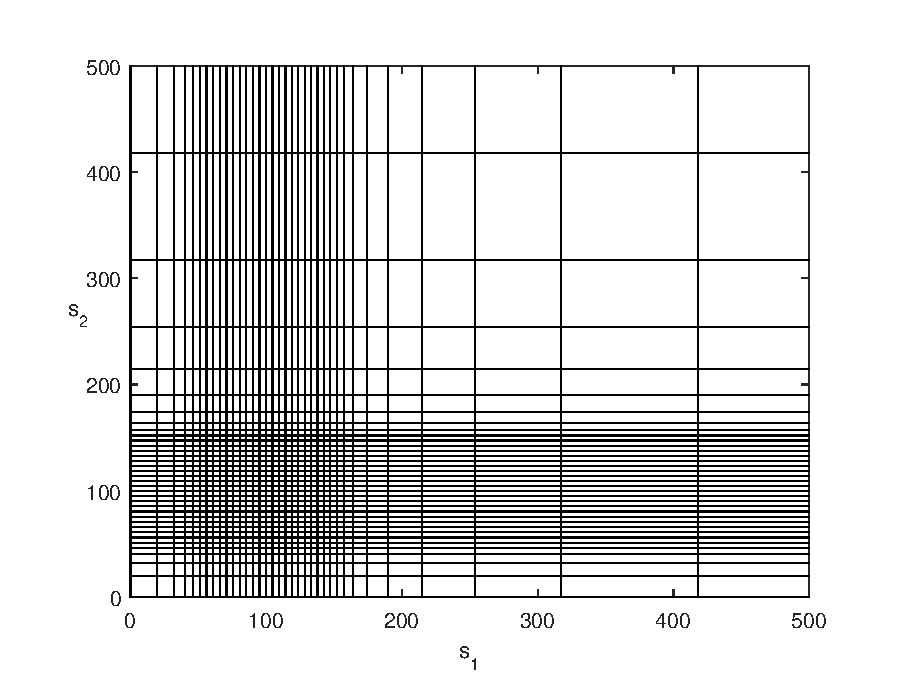
\includegraphics[scale=0.5]{Grid2DBS.eps}  
\caption{Illustration of the non-uniform grid around $(S_{1,0},S_{2,0})$ for the actual values $S_{1,0}=S_{2,0}=100$, $m_{1}=m_{2}=40$.}
\label{fig:Grid2DBS}
\end{center}
\end{figure}
The FV discretization from Subsection \ref{2DKolmogorov} then defines approximations $P_{i,j}(\tau)$ to $p(s_{1,i},s_{2,j},\tau)$ and we compute the total spatial error
$$ \max_{1 \le i \le m_{1}, 1 \le j \le m_{2}} \vert p(s_{1,i},s_{2,j},T) - P_{i,j}(T) \vert. $$
In Figure \ref{fig:Convergence2DBS} the total spatial error is shown for the realistic parameter values $r= 0.03$, $\sigma_{1,BS}=0.2$, $\sigma_{2,BS}=0.25$, $T=1$ and for the number of spatial grid points $m_{1}=m_{2} = \{20,40, \ldots, 200 \}$. 
Initially, for low values of $m_{1},m_{2}$, the convergence plot indicates that the method has an order of convergence between one and two with respect to the initial-boundary value problem under consideration. For larger values of $m_{1},m_{2}$, however, it is readily seen that that the method is second-order convergent. 
\begin{figure}
\begin{center}
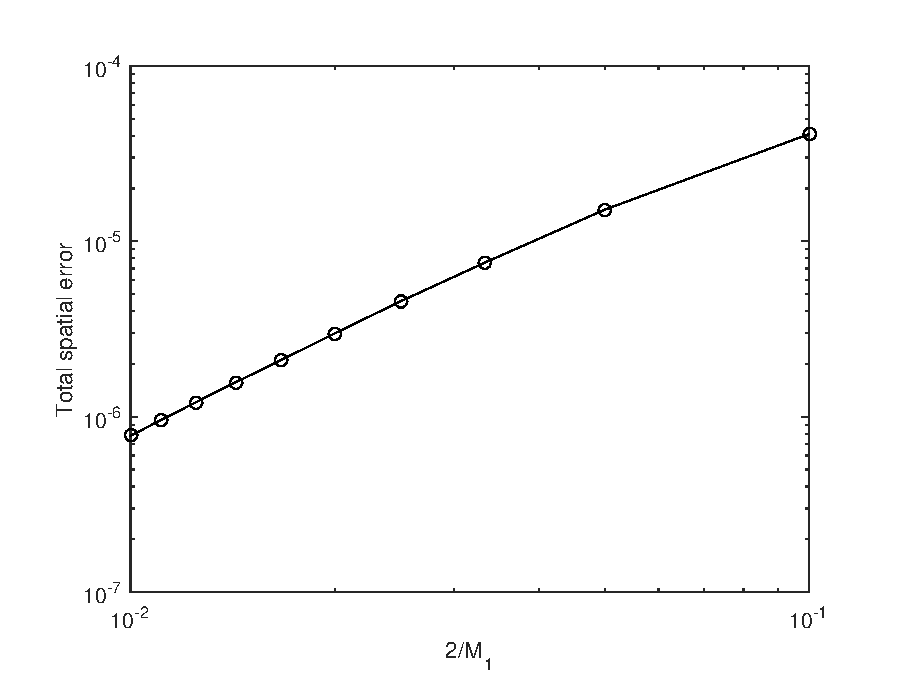
\includegraphics[scale=0.5]{Convergence2DBS.eps}  
\caption{Convergence plot for the parameter values $r = 0.03, \sigma_{1,BS} = 0.2, \sigma_{2,BS}=0.25, T=1$.}
\label{fig:Convergence2DBS}
\end{center}
\end{figure}










 




%%%%%%%%%%%%%%%%%%%%%%%%%%%%%%%%%%%%%%%%%%%%%%%%%%%%%%%%%%%%%%%%%%%%%%%%%%%%%%%%%%%%
%%%%%%%%%%%%%%%%%%   SECTION 5   %%%%%%%%%%%%%%%%%%%%%%%%%%%%%%%%%%%%%%%%%%%%%%%%%%%
%%%%%%%%%%%%%%%%%%%%%%%%%%%%%%%%%%%%%%%%%%%%%%%%%%%%%%%%%%%%%%%%%%%%%%%%%%%%%%%%%%%%
\setcounter{equation}{0}
\section{Numerical experiments}\label{Experiments}






%%%%%%%%%%%%%%%%%%%%%%%%%%%%%%%%%%%%%%%%%%%%%%%%%%%%%%%%%%%%%%%%%%%%%%%%%%%%%%%%%%%%%
%%%%%%%%%%%%%%%%%   SECTION ACKNOWLEDGEMENTS   %%%%%%%%%%%%%%%%%%%%%%%%%%%%%%%%%%%%%%
%%%%%%%%%%%%%%%%%%%%%%%%%%%%%%%%%%%%%%%%%%%%%%%%%%%%%%%%%%%%%%%%%%%%%%%%%%%%%%%%%%%%%
\setcounter{equation}{0}
\section*{Acknowledgements} 
This work has been supported financially by a PhD Fellowship of the Research Foundation--Flanders.


\vfill\eject
\begin{thebibliography}{99}

\bibitem{AP06} \textsc{Andersen, L.~B.~G., Piterbarg, V.~V.} (2007)
Moment explosions in stochastic volatility models.
\textit{Finance Stoch.}, \textbf{11}, 29--50.

\bibitem{C11} \textsc{Clarke, I.~J.} (2011)
\textit{Foreign Exchange Option Pricing: A Practitioner's Guide.}
John Wiley \& Sons.

\bibitem{CS88} \textsc{Craig, I.~J.~D., Sneyd, A.~D.} (1988)
An alternating-direction implicit scheme for parabolic equations
with mixed derivatives.
\textit{Comp. Math. Appl.}, \textbf{16}, 341--350.

\bibitem{D94} \textsc{Dupire, B.} (1994)
Pricing with a smile. 
\textit{RISK}, \textbf{7}, 18--20.

%\bibitem{ET11} \textsc{Ekstr\"om, E., Tysk, J.} (2011)
%Boundary conditions for the single-factor term structure equation.
%\textit{Ann. Appl. Prob.}, \textbf{21}, 332--350.

\bibitem{G86} \textsc{Gy\"ogny, I.} (1986)
Mimicking the one-dimensional marginal distributions of processes having an Ito differential.
\textit{Probab. Th. Rel. Fields}, \textbf{71}, 501--516.

\bibitem{IHF10} \textsc{in~'t~Hout, K.~J., Foulon, S.} (2010)
ADI finite difference schemes for option pricing in the Heston model
with correlation.
\textit{Int. J. Numer. Anal. Mod.}, \textbf{7}, 303--320.

\bibitem{IHM11} \textsc{in~'t~Hout, K.~J., Mishra, C.} (2011)
Stability of the modified Craig--Sneyd scheme for
two-dimensional convection-diffusion equations with mixed
derivative term.
\textit{Math. Comp. Simul.}, \textbf{81}, 2540--2548.

\bibitem{IHM13} \textsc{in~'t~Hout, K.~J., Mishra, C.} (2013)
Stability of ADI schemes for multidimensional diffusion equations
with mixed derivative terms.
\textit{Appl. Numer. Math.}, \textbf{74}, 83--94.

\bibitem{IHW09} \textsc{in~'t~Hout, K.~J., Welfert, B.~D.} (2009)
Unconditional stability of second-order ADI schemes applied to
multi-dimensional diffusion equations with mixed derivative terms.
\textit{Appl. Numer. Math.}, \textbf{59}, 677--692.

\bibitem{IHW15} \textsc{in~'t~Hout, K.~J., Wyns, M.} (2016)
Convergence of the Modified Craig--Sneyd scheme for two-dimensional convection-diffusion equations with mixed derivative term.
\textit{J. Comp. Appl. Math.}, \textbf{296}, 170--180.

\bibitem{HV03} \textsc{Hundsdorfer, W., Verwer, J.~G.} (2003)
\textit{Numerical Solution of Time-Dependent Advection-Diffusion-Reaction Equations.}
Berlin: Springer.

\bibitem{L02} \textsc{Lipton, A.} (2002)
The vol smile problem.
\textit{RISK}, February, 61--65.

\bibitem{M14} \textsc{Mishra, C.} (2014)
\textit{Stability of Alternating Direction Implicit Schemes with Application to Financial
Option Pricing Equations}.
PhD thesis, University of Antwerp.

\bibitem{PVF03} \textsc{Pooley, D.~M., Vetzal, K.~R., Forsyth, P.~A.} (2003)
Convergence remedies for non-smooth payoffs in option pricing.
\textit{J. Comp. Finan.}, \textbf{6}, 25--40.

\bibitem{R84} \textsc{Rannacher, R.} (1984)
Finite element solution of diffusion problems with irregular data.
\textit{Numer. Math.}, \textbf{43}, 309--327.

\bibitem{T11} \textsc{Tachet, R.} (2011)
\textit{Non-parametric model calibration in finance.}
PhD thesis, Ecole Centrale Paris.

\bibitem{TF10} \textsc{Tataru, G., Fisher, T.} (2010)
Stochastic local volatility.
\textit{Technical report, Bloomberg}.

\bibitem{TR00} \textsc{Tavella, D., Randall, C.} (2000)
\textit{Pricing Financial Instruments: The Finite Difference Method.}
New York: John Wiley \& Sons.

\bibitem{W16} \textsc{Wyns, M.} (2016)
Convergence analysis of the Modified Craig--Sneyd scheme for two-dimensional 
convection-diffusion equations with nonsmooth initial data.
Submitted for publication.

\end{thebibliography}

\end{document}
